\section{The Large Hadron Collider at CERN}

\begin{figure}[htbp]
  \centering

  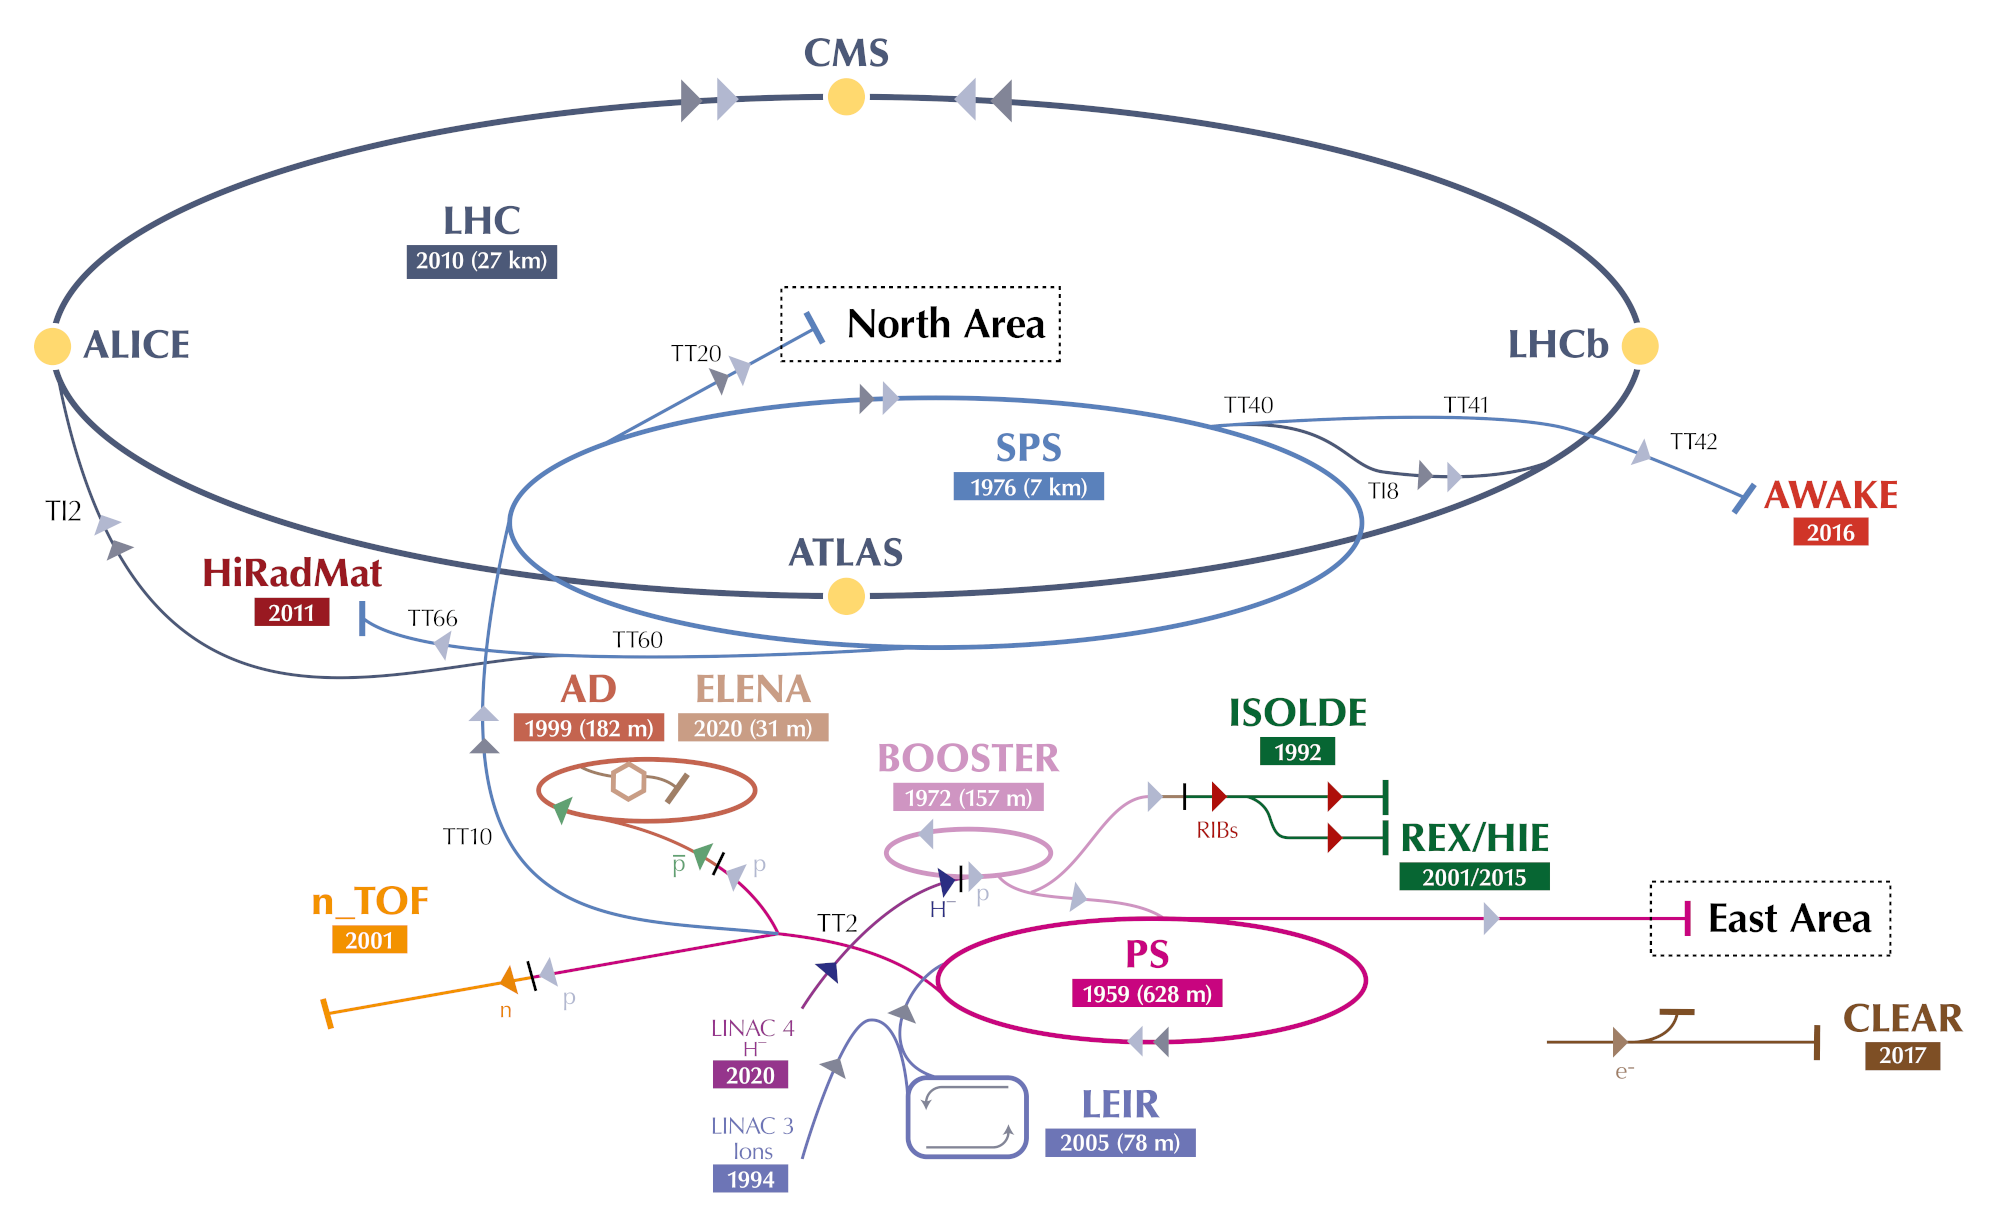
\includegraphics[width=0.9\textwidth, trim=10.5cm 44cm 2cm 20cm,
  clip]{cern_complex}

  \caption{The CERN accelerator complex in August 2018. Image adapted from
    Ref.~\cite{Mobs:2684277}.}%
  \label{fig:bla}
\end{figure}

Notes:
\begin{itemize}

\item Large Hadron Collider~\cite{Evans:2008zzb}: Geneva, Switzerland / CERN

\item Proton \& Heavy Ion Collider; ca.\ \SI{26.7}{\kilo\metre} circumference
  (underground)
  \begin{itemize}

  \item Synchrotron: 1232 dipoles (superconducting) / quadrupole magnets for
    focussing of the beam

  \item Two proton beams circulating in opposite directions.

  \item Accelerator chain (\pp): LINAC 2 (\textbf{LIN}ear \textbf{AC}celerator)
    -> Proton Synchrotron Booster -> Proton Synchrotron (PS) -> Super Proton
    Synchrotron (SPS) (injection energy of \SI{450}{\GeV})-> LHC



  \end{itemize}

\item Provides high-energy particle collisions for four large scale experiments:
  ATLAS, CMS~\cite{CMS-CMS-00-001}, ALICE~\cite{ALICE:2008ngc}, and
  LHCb~\cite{LHCb:2008vvz}; Smaller experiments?  MOEDAL~\cite{MoEDAL:2009jwa},
  TOTEM~\cite{TOTEM:2008lue}

\item Run history (time?): Run 1 \SI{7}{\TeV} (2010--2011) / \SI{8}{\TeV}
  (2012); Run 2 \SI{13}{\TeV} (2015--2018); Run 3 \SI{13.6}{\TeV} (2022--)

\item Performance characteristics of the \pp operation of the LHC during Run~2:
  \begin{itemize}
  \item Bunches \& Bunch spacing: 2556 (\SI{25}{\nano\second}) -- but 2808 RF
    buckets (not all filled)
  \item Protons per bunch: \num{1.1e11}
  \item Luminosity: \SI{2.1e34}{\per\centi\metre\squared\per\second} (design:
    \SI{1.0e34}{\per\centi\metre\squared\per\second})
  \item $\sqrt{s} = \SI{13}{\TeV}$
  \item Pile-up?
  \item Delivered integrated luminosity: about \SI{160}{\ifb}
  \end{itemize}

\item How does Luminosity relate to event rate / pile-up?
  \begin{align*}
    \frac{\mathrm{d}N}{\mathrm{d}t} = L \sigma
  \end{align*}
  Inelastic \pp cross-section at $\sqrt{s} = \SI{13}{\TeV}$ ca.\
  \SI{80}{\milli\barn}~\cite{STDM-2015-05}.

\end{itemize}

% Luminosity or pile-up plots?
% https://twiki.cern.ch/twiki/bin/view/AtlasPublic/LuminosityPublicResultsRun2

%%% Local Variables:
%%% mode: latex
%%% TeX-master: "../../phd_thesis"
%%% End:
